\section{A common geometric and symbolic toolkit}
\label{sv:toolkit}

The constructions share two interfaces: transverse pulses realize finite
rectangle maps, and local inverse rules make the rectangle families
separated. We first specify the profiles and paths used by the pulses,
then the positional coding that converts a finite rule table into their
input. The recorder itself is introduced in Section~\ref{sv:periodic-compiler}.

\subsection{Profiles that preserve the exact shear paths}
\label{sv:profiles}
Write $X(a)(x,y)=(x+ay,y)$ and $Y(a)(x,y)=(x,y+ax)$.
Besides the four shears in Theorem~3.2 of~\cite{Entry}, we will use
these chronological lists about a branch center:
\begin{align}
 &Y(-r),\ X(r^{-1}-1),\ Y(1),\ X(r-1),\label{sv:list-a}\\
 &Y(-r(r-1)),\ X(-r^{-1}),\ Y(r-1),\ X(1),\label{sv:list-b}\\
 &X(r^{-1}-1),\ Y(1),\ X(r-1),\ Y(-r^{-1}).\label{sv:list-c}
\end{align}
All have product $\operatorname{diag}(r,r^{-1})$, with products
taken in reverse chronological order.  For example, the leftmost three
factors of the full product in \eqref{sv:list-b} multiply to
$\left(\begin{smallmatrix}r&0\\r-1&r^{-1}\end{smallmatrix}\right)$;
right multiplication by $Y(-r(r-1))$ finishes the identity.
For \eqref{sv:list-c} the rightmost three factors are
$\left(\begin{smallmatrix}r&0\\1&r^{-1}\end{smallmatrix}\right)$,
which the final shear makes diagonal.

If $r,r^{-1}\le B$ and initial half-sides are at most $\ell/2$,
the crude bounds for every partial shear are
$(1+B)^4\ell/2$ for \eqref{sv:list-a},\eqref{sv:list-c}, and
$(1+B^2)^4\ell/2$ for \eqref{sv:list-b}.  Each follows by four
applications of $\|X(a)\|_\infty,\|Y(a)\|_\infty\le1+|a|$;
partial pulse coefficients have smaller modulus.  For
\eqref{sv:list-a}, the stronger endpoint-size estimate of
Theorem~3.2 of~\cite{Entry} bounds offsets by $3\ell/2$ whenever
both the source and target sides are at most $\ell$, independently
of $r$.  These estimates are useful for different chart choices.

Here are three interchangeable ways to impose zero mean while retaining
the specified paths.  A box cutoff always equals one on a neighborhood of
the indicated closed box, and is supported in a rational collar.  For an
explicit convention set $E(s)=e^{-1/s}$ for $s>0$ and zero otherwise,
and $H(s)=E(s)/(E(s)+E(1-s))$.  For $I=[a,b]$ use
\[
 \chi_{I,\delta}(s)=
 H\bigl(2(s-a+\delta)/\delta\bigr)
 H\bigl(2(b+\delta-s)/\delta\bigr).
\]
It is one on $[a-\delta/2,b+\delta/2]$, supported in
$[a-\delta,b+\delta]$, and symmetric about the interval center.
Products give box cutoffs.  Positive-side derivatives of $E$ are
polynomials in $1/s$ times $e^{-1/s}$, and the bound
$e^{-1/s}\le n!s^n$ gives effective flatness at zero to every order.
The denominator of $H$ is at least $e^{-2}$.  Thus these profiles
and all their derivatives can be evaluated without deciding equality
with a cutoff endpoint.
\begin{enumerate}
\item A rectangle selector may be
$\partial_x((x-c_x)\chi_P(x,y))$, and a height selector may be
$\partial_z((z-z_i)\zeta_i(z))$.  They equal one on their
plateaus and have integral zero by periodic differentiation.
\item A selector may be $\chi_P(x,y)-\chi_P(x,y-\delta)$,
or $\zeta_i(z)-\zeta_i(z-\delta)$, when the translated support
misses all tracked rectangles or heights.  Equal translated integrals
cancel.  A mean-zero height selector makes every supported horizontal
linear profile have zero spatial mean, even if that linear profile
does not itself have zero mean.
\item With an even local cutoff, the periodic local function
$\Xi_c(s)=(s-c)H(2-2(s-c)^2/D^2)$ is odd about $c$, hence has
zero mean.  Its derivative also has zero mean.  On $|s-c|\le D/2$
they equal $s-c$ and $1$, respectively.  Alternatively,
$\partial_s(\tfrac12(s-c)^2\chi(s))$ and
$\partial_s(s\chi(s))$ give the same linear and constant plateaus.
\end{enumerate}
All profiles are extended periodically only across a region where they
vanish.  The first recipe requires a neighborhood plateau because a
derivative is taken; the second only requires the explicit separation
from translated supports.

\subsection{The seven-stage construction and its pulse convention}
\label{sv:reciprocal-template}
The reciprocal theorem in Section~\ref{sv:imports} uses a source
selector to assign each rectangle its own height, performs its planar
map there, and uses a target selector to return it to the coding height.
We write the fields from its proof~\cite[Theorem~3.2]{Entry} in a form
allowing separate shear and translation selectors, since later
constructions change individual profiles or stages.

Write the centers of $P_i,Q_i$ as $c_i^-,c_i^+$ and the prescribed
linear part as $\operatorname{diag}(r_i,r_i^{-1})$.  Let $z_0$ be
the coding height.  Choose smooth periodic selectors $A_i^-,A_i^+$
with zero planar mean, equal to one near their own source or target
rectangle and zero near all other rectangles of the same family.
Choose distinct private heights $z_i$.  Two height selectors
$\sigma_i,\tau_i$ equal one near $z_i$ and zero near every other
private height.  Require $\tau_i$ to have zero mean.  For $j=1,2$,
choose a periodic profile $g_{ij}$ equal to $s-c_{ij}^-$ on a
neighborhood of the coordinate range of the four centered shear paths,
and require
\[
 \left(\int\sigma_i\right)\left(\int g_{ij}\right)=0.
\]
Thus the shear selector $\sigma_i$ may have nonzero mean when both
linear profiles have zero mean.  Usually one can take
$\sigma_i=\tau_i$.  The derivative, odd-profile, and translated-copy
recipes above provide these choices; their compensating parts must
miss the other tracked rectangles or private-height plateaus as
specified there.

For the chronological shear list~\eqref{sv:list-a}, the seven spatial
fields are
\begin{align}
 W_1&=e_z\sum_i(z_i-z_0)A_i^-(x,y),\notag\\
 W_2&=e_y\sum_i(-r_i)\sigma_i(z)g_{i1}(x),&
 W_3&=e_x\sum_i(r_i^{-1}-1)\sigma_i(z)g_{i2}(y),\notag\\
 W_4&=e_y\sum_i\sigma_i(z)g_{i1}(x),&
 W_5&=e_x\sum_i(r_i-1)\sigma_i(z)g_{i2}(y),\notag\\
 W_6&=\sum_i\tau_i(z)(c_i^+-c_i^-,0),\notag\\
 W_7&=e_z\sum_i(z_0-z_i)A_i^+(x,y).
 \label{sv:seven-fields}
\end{align}
At each stage all branch contributions have the same direction of
motion, except in $W_6$, whose two horizontal components depend only
on height.  Consequently each entire stage is transverse, even where
profile supports overlap.  The stated integral conditions give zero
spatial mean to every summand and hence to each $W_j$.

To turn the stages into smooth motion, choose successive closed
rational intervals $[a_j,b_j]$ with $0<a_j<b_j<1$ and positive gaps,
and set
\begin{equation}\label{sv:pulse-convention}
 \beta_j(t)=\frac1{b_j-a_j}
 H'\!\left(\frac{t-a_j}{b_j-a_j}\right),\qquad
 U(t,x)=\sum_j\beta_j(t)W_j(x)\quad(0\le t\le1).
\end{equation}
The step function $H$ defined above is nondecreasing, so each pulse
is nonnegative, has integral one, and vanishes to every order at its
endpoints.  The finite list repeats smoothly with period one and zero
collars at integer times.  This convention applies to any finite number
of repeated stages below.  The same pulse formula is used on a
separately specified finite loading interval.  Its derivatives and
their bounds are effective by the same flat-profile estimates.  Distinct stages have disjoint temporal
supports; branch contributions within one stage act simultaneously.
Thus the summed velocity still has zero self-advection, and
Lemma~\ref{sv:force} applies.

Here is the exact path represented by these fields.  Starting from
$(y,z_0)$ with $y\in P_i$, $W_1$ lifts the point to $(y,z_i)$.
Only the $i$th height selectors act during the next five stages.
The four shears send the offset $y-c_i^-$ to
$\operatorname{diag}(r_i,r_i^{-1})(y-c_i^-)$, still based at
$c_i^-$.  The sixth stage translates that center to $c_i^+$, and
$W_7$ lowers the resulting point of $Q_i$ back to $z_0$.
Nonnegative pulse masses parameterize each partial shear or translation
by a number in $[0,1]$.  The excursion estimates above therefore
verify the linear plateaus on the full closed source rectangle before
ODE uniqueness identifies these formulas with the actual trajectories.
Positive plateau margins also permit a sufficiently small neighborhood
of that rectangle and coding height; its size must be chosen from the
margins and the affine partial maps.  The bounds for points on the
original rectangle are not automatically bounds for that neighborhood.

The other four-shear lists replace $W_2,\ldots,W_5$ by their listed
coefficients and directions, using their own excursion estimates.
Splitting $W_6$ into an $x$-translation and a $y$-translation gives the
eight-stage version.  If extra transverse controls are used, the first
is one on the current $y$-interval and the second on the target
$x$-interval already reached; both retain the private-height selector.
Their scalar coefficients must have zero integral, supplied by either
factor or by a correction supported off every tracked path.  Remote
centers and routes with an extra translation are specified separately
below: their endpoint maps use the same principles, while their
intermediate paths require the bounds proved for those routes.


\subsection{A digit interface for full rule domains}
\label{sv:digits}
A relative tape is a bi-infinite sequence $T=(T_j)_{j\in\mathbb Z}$
whose index zero is the current head position. If an edit produces
$\widetilde T$, displacement $d$ gives $T'_j=\widetilde T_{j+d}$.
A full cylinder fixes a mode and finitely many tape letters, with every
other letter arbitrary. This convention specifies the domains on which
we will prove local inverses.

Let an alphabet of size $m$ have distinct digits separated by at least two
in base $B$, with all digits in $\{0,\ldots,B-2\}$.  Write
\[
 C(a_1a_2\cdots)=\sum_{j\ge1}d(a_j)B^{-j},\qquad
 I(v)=\left[\sum_{j=1}^{|v|}d(v_j)B^{-j},
 \sum_{j=1}^{|v|}d(v_j)B^{-j}+B^{-|v|}\right].
\]
The two coordinates of a relative tape are $C(T_{-1}T_{-2}\cdots)$
and $C(T_0T_1\cdots)$.  Place the modes in pairwise positively separated translated squares of
common side length $\ell$, and use these two codes as the coordinates
within each square.  This is the positional-coding principle of
Moore~\cite{Moore1991}; the following lemma records the full-rectangle
and separation properties used here.

\begin{lemma}[Full cylinders give full rectangles]\label{sv:full-cylinders}
Suppose a finite injective partial rule map is partitioned into full
cylinders specified by a mode and the tape window $[-a,b-1]$.  A branch
edits only that window and shifts by $d$, with $a+d,b-d\ge0$.
Its image cylinder has the rewritten prefixes of lengths $a+d,b-d$.
The associated closed source and target rectangles are separately
pairwise separated.  The exact branch map on the whole rectangle has
linear part $\operatorname{diag}(B^{-d},B^d)$.
\end{lemma}
\begin{proof}
A prefix $v$ followed by an arbitrary tail has code
$C(v)+B^{-|v|}C(\text{tail})$.  The two free tails survive the edit and
shift, so changing prefix lengths gives the stated affine factors on all
tail parameters in $[0,1]$.  Thus each image really is a full cylinder.
If two cylinders in one mode are disjoint, their left prefixes or their
right prefixes must be incompatible; otherwise arbitrary compatible
extensions would give a common tape.  At the first differing digit of
incompatible words, their intervals have a positive gap, at least the
corresponding digit scale.  This proves source separation and, by
injectivity, target separation.  Distinct mode squares are separated by
their placement.  A constant tail has rational code
$B^{-k}d(a)/(B-1)$ after a prefix of length $k$; therefore all finite
input codes are rational and effectively known.  Positive gaps allow
successive finite-prefix decoding from promised codes, including codes
on rectangle boundaries.
\end{proof}

For a single-cell table there is a shorter sufficient inverse test: the
target mode determines the incoming displacement, and the target mode
together with the written letter determines the old mode and old letter.
One first reverses the displacement, then the unique write.  Let
$T_a(v)=(d(a)+v)/B$ and $I_a=T_a([0,1])$.  Reading $a$, writing $b$,
and moving by $d$ gives the following complete rectangle formulas:
\begin{equation}\label{sv:single-cell-maps}
\begin{array}{c|c|c|c}
d&\text{source}&(L',R')&\text{target}\\\hline
1 &[0,1]\times I_a &(T_b(L),T_a^{-1}(R))&I_b\times[0,1]\\
0 &[0,1]\times I_a &(L,T_bT_a^{-1}(R))&[0,1]\times I_b\\
-1&I_c\times I_a &(T_c^{-1}(L),T_cT_bT_a^{-1}(R))
 &[0,1]\times T_c(I_b).
\end{array}
\end{equation}
Include the last row for every $c$.  Determinism separates sources.
The inverse test separates target written letters; in the last row the
pair $(c,b)$ separates the two-digit target intervals.  If mode-square
gaps are at least $\ell$, all within-family gaps are at least
$\ell/B^2$ in one coordinate.

\paragraph{Common force conclusions.}
In each construction below choose nonnegative smooth unit-integral
pulses strictly inside the listed phases and repeat their finite list
with period one.  The velocity is zero near integer times, so the
initial velocity is zero.  Every fixed mixed derivative of the force
and velocity is bounded, and the kinetic energy is uniformly bounded.
The force is effective for computable $\nu>0$, and the same formula is
effective relative to an arbitrary supplied positive viscosity.
Unless stated otherwise, $m$ is the augmented tape alphabet size,
$N$ the recorder mode count, $J$ the number of rectangle branches,
and $(L_*,R_*)$ the rational initialized left and right codes.

\section{A compiler periodic from time zero}
\label{sv:periodic-compiler}

We now prove Theorem~\ref{sv:periodic-theorem}. The recorder below retains
each instruction before moving the simulated head. Its full-domain inverse
provides separated rectangle maps; two ways of incorporating the input
then make the entire pulse schedule periodic from time zero. A separate
one-time loader would give only eventual periodicity.

Throughout the recorder constructions a machine instruction indexed by $i=(q,a)$ has
data $(q_i,b_i,d_i)$, where $d_i\in\{-1,0,1\}$.  Missing instructions
may be completed by unchanged-symbol, zero-displacement moves to a halt
state.  Every table below is partial: an unlisted case
has no rule. On initialized tapes, all auxiliary tracks are blank away
from the specified finite initialization, and all unspecified mark bits
are zero. The full partial domains are restricted only by the displayed
local guards.

When an idle nonhalting start is requested, add a fresh state with one
unchanged-symbol, zero-displacement instruction for each tape letter,
leading to the original start state. No instruction targets the fresh
state. This adds one simulated step, preserves halting even when the
original start is already halted, and leaves the initial tape unchanged.

\subsection{Recording before the simulated move}
\label{sv:old-head}\label{sv:periodic-options}
This recorder marks the old head, logs the instruction, and only
then makes the simulated move.  Let $e\in\{-1,0,1\}$ remember the
preceding move, let $r=(q,e,a)$, and give its instruction the data
$(q_r,b_r,d_r)$.  Letters are $(a,h,m)$, with
$h\in\{E,F\}\sqcup\{r\}$ and $m\in\{0,1\}$.  The controls are
$M_{q,e},R_r,P_{q,d},L_{q,d}$.  The following table uses $h\ne F$:
\begin{equation}\label{sv:old-head-table}
\begin{array}{c|c|c|c|c}
\text{source}&\text{read}&\text{written}&\text{move}&\text{target}\\\hline
M_{q,e}&(a,h,0)&(b_r,h,1)&1&R_r\\
R_r&(c,h,0)&(c,h,0)&1&R_r\\
R_r&(c,F,0)&(c,r,0)&1&P_{q_r,d_r}\\
P_{q,d}&(c,E,0)&(c,F,0)&-1&L_{q,d}\\
L_{q,d}&(c,h,0)&(c,h,0)&-1&L_{q,d}\\
L_{q,d}&(c,h,1)&(c,h,0)&d&M_{q,d}.
\end{array}
\end{equation}
Only nonhalting $q$ have a first row.  Initialize the frontier at
absolute cell $c_0$, where either $c_0=1$ or $c_0=2$, and start in
$M_{q_0,0}$.  At the $n$th main visit the head is the machine head
$h_n$, the records occupy $c_0,\ldots,c_0+n-1$, and the frontier is
$J_n=c_0+n$.  Since $h_n\le n<J_n$, the first row is defined.
It marks $h_n$, the right scan logs at $J_n$, the placement row moves
the frontier to $J_n+1$, and the left scan returns to the unique mark.
The last row makes the original move.  This is exactly
$2(J_n-h_n)+3$ local steps, a finite positive number; for $c_0=2$
it lies between $7$ and $4n+7$.  Thus main halts and original halts
agree, with no intervening main visit.

This table also passes the inverse test on arbitrary tapes.  Into $R_r$,
the written mark distinguishes entry from its loop and $r$ recovers
the old work symbol and control.  Into $P$, the written record identifies
the predecessor.  Into $L$, a written frontier distinguishes placement
from scanning.  Into $M_{q,d}$, the sole predecessor restores a mark and
has known displacement $d$.  All other tracks are retained.  Incoming
displacements are respectively $1,1,-1,d$, proving the test.

The choices $c_0=1$ and $c_0=2$ have the same entire rule table but
different initialized histories.  A permanent origin bit may be added
and copied by every rule.  When $c_0=1$ without such a bit, the leftmost
nonempty history cell remains absolute cell one and also determines
absolute indexing.  These are precise ways of recovering the head
position, rather than additional assumptions on arbitrary tapes.

\paragraph{An old-head recorder with an input-shifted chart.}
Use \eqref{sv:old-head-table} with frontier at two and an idle
nonhalt start.  Put $\ell=1/(64N(1+B)^4)$, with odd digits in
base $B=2m+1$.  The initial origin is
$(1/4-\ell L_*,1/2-\ell R_*)$; other nonhalt origins are
$(1/4+2j\ell,1/2)$ for $j\ge1$, and halt origins are
$(5/8+2j\ell,1/2)$ with a fresh enumeration.  All squares remain
separated, and nonhalt centers have first coordinate at most $9/32$.
Use collars $\ell/(10B^2)$, selectors corrected by a $1/4$ shift
in $y$, and heights $1/2+i/(8(J+1))$ with collar
$1/(32(J+1))$, corrected by a $1/4$ shift in $z$.
The seven phases with \eqref{sv:list-a} have excursion
$1/(128N)$ inside $[1/8,7/8]$.  Nonhalt paths have $x<1/2$;
halt endpoints lie in $[5/8,21/32]$.  The label is
$(1/4,1/2,1/4)$ and the fixed event is $1/2<x<7/8$.

There is a second exact specialization of the same rule table: put the
frontier at one, use odd digits in base $B=2m+2$, set
$\ell=1/(64(N+1))$, and use the same initial-chart shift and other
origins.  Use derivative rectangle and height masks and the endpoint-size
bound $3\ell/2$, which does not grow with $B$.  The label remains
$(1/4,1/2,1/4)$ and the event can be narrowed to $1/2<x<3/4$.
Indeed nonhalt paths satisfy
$x\le1/4+2N\ell+3\ell/2<1/2$, while halt endpoints lie
in $[5/8,5/8+2N\ell]\subset(1/2,3/4)$.
This preserves the different initialized history and observer without
repeating the six-rule inverse proof.

\paragraph{A reserved loading target.}
Instead make a fresh copy $q_0$ of the original start state, preserving
its halting status, and arrange that no instruction targets this copy.
In \eqref{sv:old-head-table}, retain placement and return controls only
for state-displacement pairs that occur as instruction targets.
No rule then enters $M_{q_0,0}$.  For $N$ remaining modes set
$\ell=1/(32(N+1)(1+B)^4)$ and put their origins at
$(1/4+2j\ell,1/4)$ or $(5/8+2j\ell,1/4)$ according to
halting status.  The initial code $q^{\rm in}$ has coordinate margins
at least $\ell/(B-1)$ inside its mode square.  Add a translation
from the square centered at $(1/4,1/2)$ with half-width
$\ell/(4(B-1))$ to the congruent square at $q^{\rm in}$.
Its source is separated in $y$; its target is inside a square having
no incoming rule.  Thus both augmented families are separated.
Use eight phases with \eqref{sv:list-a}, derivative rectangle masks,
and local profiles $\Xi_c$ with $D=1/16$.  The excursion
$(1+B)^4\ell/2<1/32$ fits every plateau; use a collar at most
one quarter of $\min(1/32,\ell/B^2,1/(4(J+1)))$.
For nonhalting loading and later transitions,
$x\le5/16+(1+B)^4\ell/2<1/2$; halt targets lie in
$[5/8,11/16)$.  The label and event are again
$(1/4,1/2,1/4)$ and $1/2<x<7/8$.  Initially halted inputs
hit during the first loading period.  The loader remains in the repeated
table, so periodicity begins at zero.

\begin{proof}[Completion of Theorem~\ref{sv:periodic-theorem}]
The input-shifted chart gives all the stated force and event properties.
The reserved loading branch gives the same fixed label and observer,
with eight axial phases and hence one Cartesian component at a time.
Both satisfy Lemma~\ref{sv:force}; their rational parameters and
effective flat profiles give the stated derivative evaluation.
\end{proof}

\section{Alternative recorder contracts}
\label{sv:recorders}

The headline compiler is complete. The alternatives in this section
change what information is present at initialization or at a return to
an ordinary machine state. Their local guards matter: each inverse must
hold on every allowed tape, including tapes outside the initialized run.
Instruction histories retain the information needed for reversibility
\cite{Bennett1973}; the rules below specify how that information is
recovered in each case.

Section~\ref{sv:tagged-initializer} writes a finite input from an entirely
blank tape inside the repeated table. Section~\ref{sv:guarded} trades a
neighbor guard for shorter history updates and then keeps a persistent
head mark. Section~\ref{sv:remote} uses that mark for a reserved loader
and an exact map on a box of positive thickness.
Section~\ref{sv:head-origin} combines the work and departure steps while
retaining an origin flag. Each rule table is followed by its inverse,
its initialized simulation, and a geometric realization with a fixed
observer; these are different guarantees rather than extra steps in
the proof of Theorem~\ref{sv:periodic-theorem}.

\subsection{Writing the input inside the repeated rule table}
\label{sv:tagged-initializer}
A one-time loader gives eventual periodicity.  To keep periodicity from
time zero, the loading operation can instead be a distinguished local
branch.  Here is a version starting from an entirely blank tape.
Let $r=(q,e)$, with $e\in\{-1,0,1,\star\}$; only initialization
uses $\star$.  For a nonhalt instruction put $k=(r,a)$,
$s(k)=(q',d)$.  Letters are $(a,m,g)$ with
$g\in\{E,P\}\sqcup\{k\}$; modes are $I,C_r,S_k,B_s$.
\begin{enumerate}
\item In $I$ require cells $0,\ldots,R_0-1$ fully blank, where
$R_0=\max(2,|w|)$.  Write the input and a history pointer at cell one,
and enter $C_{(q_0,\star)}$ without moving.
\item In nonhalt $C_r$ require $m_0=0,g_0\ne P$; write the
instruction symbol, mark cell zero, move right into $S_k$.
\item In $S_k$ require $m_0=0$.  Scan right if $g_0\ne P$;
if $g_0=P,g_1=E$, write $k,P$, move left into $B_{s(k)}$.
\item In $B_s$ require $g_1\ne P$.  At $m_0=0$ scan left;
at $m_0=1$ erase the mark, move by the displacement in $s$, and
enter $C_s$.
\end{enumerate}
The star tag distinguishes initialization from every other arrival in
a primary mode; it restores exactly the required blank block.  At an
$S_k$ output, the mark at $-1$ distinguishes entry and scanning.
At a $B_s$ output, the pointer at two distinguishes turning and
scanning; the record at one identifies $k$.  An ordinary primary output
has a specified return state.  These are full-domain inverse tests.
At the main visit after $n$ steps, the frontier is $n+1>h_n$ and
the records occupy $1,\ldots,n$.  The old-head shuttle therefore
takes $2(n-h_n)+3$ rules, including the final erase-and-move rule.
An initially halting machine is reached immediately after the initializer.  The
ordinary rules are resolved on $[-1,1]$, the initializer on
$[0,R_0-1]$; Lemma~\ref{sv:full-cylinders} applies to both.

\paragraph{A blank initial tape and an initialization branch.}
Use Section~\ref{sv:tagged-initializer}.  Give the fully blank symbol
digit zero, the other symbols the remaining even digits, and use
$B=2m+1$.  Set $\ell=1/(16N(1+B^2)^4)$ and enumerate modes with
$I$ first.  Their origins are $(1/4,1/4+2j\ell)$, except that
primary halt modes have first coordinate $5/8$.  The initial blank
code is $(1/4,1/4,1/4)$.  Derivative rectangle masks and the
primitive-derived linear and constant profiles above implement eight
axial phases with \eqref{sv:list-b}.  All centered excursions are at
most $1/(32N)$ and lie within $[1/8,7/8]^2$.  If the target is
nonterminal, $x\le1/4+\ell+1/(32N)<1/2$ at every phase;
halt targets have $x\in[5/8,5/8+\ell]\subset(1/2,3/4)$.
The initializer's star tag proves that its target family is disjoint
from every ordinary arrival.  Thus the fixed event is $1/2<x<3/4$,
including immediate halting after the initialization rule.

\subsection{Neighbor guards and a persistent head}
\label{sv:guarded}
Here the history append writes two adjacent cells at once.  This saves a
local step, but the inverse now needs a neighbor guard.

\paragraph{An erased return mark.}
Letters are $(a,m,g)$, with $g\in\{E,P\}\sqcup\{i\}$; controls
are $A_q,B_i,C_q$.  Use the following complete rules:
\begin{enumerate}
\item At nonhalt $A_q$, require $m_{d_i}=0$, write $a_0=b_i$,
set $m_{d_i}=1$, shift by $d_i$, and enter $B_i$.
\item At $B_i$, if $g_0\ne P$ and $m_1=0$, shift right in $B_i$.
\item At $B_i$, if $g_0=P,g_1=E$, write $g_0=i,g_1=P$,
do not shift, and enter $C_{q_i}$.
\item At $C_q$, if $m_0=0,g_0\ne P$, shift left in $C_q$.
\item At $C_q$, if $m_0=1$, erase the mark and enter $A_q$ without
shifting.
\end{enumerate}
For an output in $B_i$, the current mark distinguishes the first row
from the right scan, whose destination is guarded unmarked.  In the
first case $i$ recovers the overwritten instruction and the guard recovers
the old mark.  For an output in $C_q$, a pointer at index one identifies
the append and its record at zero identifies $i$; a left-scan output
has no pointer at index one, by its departure guard.  An output in
$A_q$ restores the erased mark.  This proves injectivity on the full
partial domain.

Initially put the pointer at two, with no marks.  After $n$ main steps
it is at $J=n+2$, and the new head $h_{n+1}\le n+1<J$.
The first rule marks that new head.  Scanning, appending, and returning
there take exactly $2(J-h_{n+1})+3$ rules.  Every guard holds; the
records occupy $2,\ldots,n+1$ at a main checkpoint.  A fresh idle
nonhalt start handles an originally halted input when the initial
particle is placed outside the observation set.

\paragraph{The three-cell guard.}
Use the erased-return-mark recorder in Section~\ref{sv:guarded}, with
an idle nonhalt start, odd digits in base $B=2m+1$, and $N$ modes.
Set $\ell=1/(100(N+1)B^6)$.  For rational initial codes $L_*,R_*$,
place the nonhalt squares, starting with the initial mode at $j=0$, at
\[
 (1/4-\ell L_*+2j\ell,\ 1/4-\ell R_*),
\]
and the halt square at $(3/4,1/4-\ell R_*)$, all of side $\ell$.
The initialized particle is $(1/4,1/4,1/4)$.  Full triple rectangles
have gaps at least $\ell B^{-3}$; choose collar $\ell/(10B^3)$.
Use the half-period difference in $y$ for their selectors.  Set
$z_i=1/2+i/(4(J+1))$ for the $J$ branches, with disjoint small
height supports.  The linear profiles may be
\[
 (s-c)\chi_{[1/8,3/8],1/32}(s)
 -(s+1/2-c)\chi_{[1/8,3/8],1/32}(s+1/2),
\]
interpreted through their local periodic charts.  They have zero mean
and equal $s-c$ in the working strip.  Use the seven phases with
\eqref{sv:list-a}.  Their excursion is less than
$(1+B)^4\ell\le16B^4\ell<0.02$.  Nonhalt source and target
squares lie in $0.24<x<0.27$, and their full period paths lie in
$0.23<x<0.28$.  Halt endpoints lie in $[3/4,0.76)$.
Consequently the fixed event $2/3<x<5/6$ is exactly halting, at all
real times.

\paragraph{Marking after a separate work step.}
Use history alphabet $\{E,F\}\sqcup\{i\}$ for this and the
next two recorders. A different six-rule map first writes and moves
without testing a mark:
at $R_q$, write $a_0=b_i$, shift $d_i$, and enter $P_i$;
at $P_i$, require $m_0=0$, set $m_0=1$, shift right into $G_i$.
In $G_i$, require $m_0=0$ and either scan right when $g_0\ne F$,
or, when $g_0=F,g_1=E$, write $g_0=i,g_1=F$, shift left into
$L_{q_i}$.  In $L_q$, scan left when $m_0=0,g_1\ne F$;
when $m_0=1$, erase it and enter $R_q$ without moving.
The outputs in $P_i$ retain the overwritten instruction.  At $G_i$,
the mark at index $-1$ distinguishes entry from scan.  At $L_q$,
the pointer at index two distinguishes append from scan, and the record
at one recovers $i$.  At $R_q$ the erased mark is restored.  Hence this
is another injective partial map.  With frontier $J=n+2$ its main
cycle has $2(J-h_{n+1})+2$ rules.  It is not identified with the
preceding map: the first rule has different guards and the append moves.

\paragraph{The two-cell append.}
For the separate-work-step map of Section~\ref{sv:guarded}, use even
digits in base $B=2m+1$ and the shorter containing interval
\[
 I(v)=[C(v),C(v)+B^{-|v|}C_*],\qquad C_*=2(m-1)/(B-1)<1.
\]
The proof of Lemma~\ref{sv:full-cylinders} applies with tail interval
$[0,C_*]$; incompatible prefixes have gap at least
$(2-C_*)B^{-j}$ at their first differing position $j$.
Put $\rho=1/(100(N+1)(B+1)^4)$,
$Y=1/2-\rho R_*$, $X_h=3/4$, and
$X_s=1/4-\rho L_*+2j(s)\rho$ for nonhalt states, starting
with the fresh idle start at $j=0$.  At coding height $1/4$, the label
is $(1/4,1/2,1/4)$.  Triple branches have gaps greater than
$\rho B^{-3}$; choose collar $\rho/(10B^3)$.
Use half-period differences in $y$ and in height, heights
$1/2+i/(8(J+1))$ with collar $1/(32(J+1))$, and
\eqref{sv:list-c}.  The excursion is at most
$(B+1)^4\rho<1/100$.  Nonhalt paths satisfy
$x<1/4+1/50+1/100<2/3$; halt endpoints are in
$[3/4,3/4+\rho]$.  Thus the event is $2/3<x<5/6$.
The unslowed force is periodic from zero.  A separate fourth-root choice
$g(t)=(1+t)^{1/4}-1$ has the same event and satisfies
$\|D_x^\alpha f(t)\|_\infty=O_\alpha((1+t)^{-3/4})$,
with all mixed derivatives bounded, by Proposition~\ref{bcs:power-clock}.
In particular every spatial derivative of the force is square integrable
in time in spatial supremum norm.  The periodic and slowed forces are
separate prescriptions.

\paragraph{A persistent head mark.}
For a third map, start with a unique mark at the machine head and retain
it at every main visit.  Use controls $C_q,D_i,R_i,L_q$, with a fresh
idle start $q_b$ which is no instruction target; omit $L_{q_b}$.
At nonhalt $C_q$ require $m_0=1$ and, if $d_i\ne0$, $m_{d_i}=0$;
write $b_i$, move the mark to $d_i$, shift $d_i$, and enter $D_i$.
At $D_i$ require $m_0=1$, shift right into $R_i$.
At $R_i$ require $m_0=0$; scan right if $g_0\ne F$, or append
$i,F$ over $F,E$ at indices $0,1$ and shift left into $L_{q_i}$.
At $L_q$ scan left when $m_0=0,g_1\ne F$; at $m_0=1$ enter
$C_q$ without editing or moving.  The inverse tests are respectively
the instruction $i$, the mark at $-1$, the pointer at two with its
record at one, and the unchanged marked tape.  Thus they apply without
assuming unique markers globally.  No rule enters $C_{q_b}$.
With the initial history end at two, the main-cycle count is
$2(J-h_{n+1})+2$.  The mark remains at the new machine head throughout
logging, and all initialized guards hold.

\subsection{A remote center and positive thickness}
\label{sv:remote}
The persistent-head recorder of Section~\ref{sv:guarded} has an
initial mode with no incoming rule.  Place its mode squares first in
unscaled coordinates: the first origin is $2j$ for a main halt and
$-2j$ for every other mode, with distinct positive indices $j$;
the second origin and coding height are zero.  Use odd digits in base
$B$ and full triples.  The rectangle gaps are at least $B^{-3}$,
and half-widths are at most $1/2$.  Let $N$ be the number of
ordinary branches plus one, let $O_0$ be the largest absolute mode
origin, and set
\[
 K=(1+B^2)^4,\qquad R=10N+O_0+K+10,\qquad L=64R.
\]
The loading branch is the translation of the square of half-width
$1/(4B)$ centered at $(-4R,0)$ to the congruent square centered
at the rational initial code.  Odd-digit codes have coordinate
margins at least $1/(B-1)$, so its target fits inside the mode
square.  That square has no incoming branch.  Both augmented rectangle
families are consequently separated.

Choose heights $Z_i=10i$, source and target collars $1/(4B^3)$,
and height cutoffs $g_i$ equal to one on $[Z_i-1,Z_i+1]$, supported
within a further unit collar.  The common center is $c^\circ=(-2R,0)$.
Use eight motions: lift by $Z_i$, translate the center to $c^\circ$,
perform \eqref{sv:list-b} there, translate to the target center,
and lower by $Z_i$.  The central linear profiles are
\[
 (X+2R)\chi_{[-K,K],1}(X+2R)g_i(Z),\qquad
 Y\chi_{[-K,K],1}(Y)g_i(Z).
\]
All scalar profiles have compact support in $(-L/8,L/8)$ in their
dependent coordinates.  For a scalar profile $a$ depending on $d$
coordinates define
\begin{equation}\label{sv:remote-correction}
 a^\#(v)=\sum_{m\in\mathbb Z^d}
 \left(a(v-Lm)-a(v-Lm-(L/2)e_1)\right).
\end{equation}
This is $L$-periodic and has zero mean.  In the central cube it
agrees with $a$, since every noncentral or negatively translated copy
is disjoint there.  Replace every scalar profile by this correction.

For every starting height $z\in[-1,1]$, lifting puts the point in
$[Z_i-1,Z_i+1]$.  The four-shear offset bound is $K/2$, with
partial coefficients included, and the two translations keep offsets
at most $1/2$.  All paths lie in $(-8R,8R)^3$; every controlling
profile remains on its intended plateau and all correction terms vanish.
The time-one map is therefore the specified reciprocal affine map on
the entire $P_i\times[-1,1]$, with the height unchanged.  This is
a neighborhood statement, not merely an assertion on the coding sheet.

Let $W$ denote the resulting $L$-periodic spatial field and
$a=(1/2,1/2,1/2)$.  At the prescribed unit-torus viscosity $\nu$,
define
\[
 U(t,x)=L^{-1}W(t,L(x-a)),\qquad
 f(t,x)=\bigl(L^{-1}W_t-\nu L\Delta W\bigr)(t,L(x-a)).
\]
The factor of the Laplacian is $L$.  These formulas directly give
zero pressure, mean-zero solenoidal forcing, and the same time period.
The loading center becomes the fixed label $(7/16,1/2,1/2)$.
During a nonhalting transition the endpoint centers are at most $-1$
in first coordinate.  Translation paths have $X\le-1+1/2<0$;
central shear paths have $X\le-2R+K<0$.  Loading obeys the same
bound, and no path crosses the chart seam.  A halt endpoint has positive
first coordinate.  Thus the fixed event on the unit torus is
$1/2<x<1$, and the loader is part of the period repeated from zero.
The locally finite sum \eqref{sv:remote-correction} is effectively
evaluated from known supports and a bounded coordinate enclosure.

\subsection{Moving the head and retaining the origin}
\label{sv:head-origin}
The persistent map admits a distinct five-rule form.  Normalize to one
halt state and a different, fresh nonhalting start.  Use a return control
$B_q$ for every $q$, including that start; this version does not impose
the preceding no-incoming-start restriction.  Add an origin
bit, fixed at absolute zero and never edited, and combine the first two
motions: at $M_q$, perform the same guarded write and mark move but
shift by $d_i+1$ into $O_i$.  The $O_i$ scan and append and the $B_q$
return and exit are the preceding $R_i,L_q$ rules.  An $O_i$ output
from the main rule has mark one at index $-1$; a scan output has mark
zero there.  The append/return distinction is still the pointer at two.
This proves the full inverse, including the possible shifts zero and
two.  At a main checkpoint the history end $J$ satisfies $J\ge h+2$.
After the work move to $h'=h+d_i$, the working cursor is $h'+1\le J$.
There are $J-1-h'$ outward and the same number of backward scan steps,
so one machine transition uses $2(J-h')+1$ rules.  The origin flag
recovers absolute indexing independently of the history.  Resolving
on $[-2,1]$ gives prefix lengths $2,2$ and target lengths $2+d,2-d$
for each actual working shift $d\in\{-1,0,1,2\}$; an empty target
prefix when $d=2$ is allowed in Lemma~\ref{sv:full-cylinders}.

The preceding three guarded recorders use complete triples on $[-1,1]$, with target
prefix lengths $1+d,2-d$.  Thus all four maps provide the full closed
rectangle interface.  The initialized marker invariant proves halting
equivalence; the separate inverse proofs prove geometric separation.

\paragraph{A head marker and a separate origin flag.}
Use the five-rule map just proved.
Set $\ell=1/(100(N+1))$, put its start origin at
$(1/4,1/4)-\ell(L_*,R_*)$, its halt origin at $(3/4,1/4)$,
and its other origins at $(1/4+(3+2j)\ell,1/4)$.
Nonhalt coordinates are at most $27/100$.  Resolve the four-cell
window and use odd digits in base $2m+1$.  The possible scale includes
$B^{-2}$, but both endpoint side lengths are at most $\ell$.
Derivative selectors and \eqref{sv:list-a} therefore have excursion
$3\ell/2$ by the endpoint-size estimate.  Every path lies in the
linear chart and a nonhalting one satisfies
$x\le27/100+3\ell/2<1/2$.  Halt endpoints lie in
$[3/4,3/4+\ell]$.  This gives the label $(1/4,1/4,1/4)$
and event $1/2<x<7/8$.

In each of these cases the rectangle identity proves the code evolution
by induction at integer times.  The recorder's positive finite cycle
counts prove that every machine step is completed.  The displayed bounds
exclude the observer during every phase of every transition whose source
and target are nonterminal.  The final transition into a terminal code
is allowed to enter the observer before its endpoint.  These facts give
the claimed equivalence at every real time, rather than merely at the
sampling times.

\section{Loading once, changing the clock, and choosing the chart}
\label{sv:reciprocal-applications}

\subsection{Onto clocks and the exact derivative estimates}
\label{bcs:clocks-section}
Slow forcing must still complete every finite logical step.  The relevant
condition is that the new clock maps the nonnegative half-line onto itself.
The following elementary calculation applies to our transverse pulse
templates, including their finite loading intervals.

\begin{lemma}[Onto clocks]\label{bcs:clock}
Let $W(s,x)$ be a smooth divergence-free field on a flat torus, with
zero mean, $W(0)=0$, bounded mixed derivatives and
$(W\cdot\nabla)W=0$.  Let $g:[0,\infty)\to[0,\infty)$ be
smooth, nondecreasing and onto, with $g(0)=0$.  Then
\begin{align*}
 u(t,x)&=g'(t)W(g(t),x),\\
 f(t,x)&=g''(t)W(g(t),x)+(g'(t))^2W_s(g(t),x)
                         -\nu g'(t)\Delta W(g(t),x)
\end{align*}
give a mean-zero solenoidal force and a solution with zero pressure and
zero initial velocity.  Its flow is $X_u(t,a)=X_W(g(t),a)$, so every
all-time reachability event is unchanged.  For $g(t)=\log(1+t)$ and
every $k,\alpha$,
\[
 \|\partial_t^kD_x^\alpha u(t)\|_\infty+
 \|\partial_t^kD_x^\alpha f(t)\|_\infty
 \le C_{k,\alpha}(1+t)^{-1-k}.
\]
All these derivatives are square integrable in time in supremum norm,
and in space--time.
\end{lemma}
\begin{proof}
The chain rule gives $f=u_t-\nu\Delta u$.  Divergence, mean zero,
and vanishing self-advection persist under multiplication by the scalar
$g'(t)$ and time composition.  The same chain rule proves the trajectory
identity by ODE uniqueness.  Onto ensures that every finite logical time
has a finite physical preimage, proving both implications for the event.
The energy comparison in Lemma~\ref{sv:force} applies to this explicit
solution on every finite interval, without a periodicity assumption.

For the logarithmic choice put $a=(1+t)^{-1}$ and $s=\log(1+t)$.
The velocity is $aW(s)$ and the force is
$-\nu a\Delta W(s)+a^2(W_s-W)(s)$.
For each positive integer $r$,
\[
 \partial_t[a^rA(s,x)]=a^{r+1}(\partial_s-r)A(s,x).
\]
Repeated differentiation and the bounded template derivatives give the
stated estimate.  Its square is integrable, and the torus has finite
volume.  These are estimates for the precomputed force formula and
require no simulation of the instructions.
\end{proof}

\begin{proposition}[Cube-root and fourth-root clocks]
\label{bcs:power-clock}
Under the hypotheses on $W$ in Lemma~\ref{bcs:clock}, choose
$g(t)=(1+t)^q-1$, with $q=1/3$ or $1/4$, and put $\beta=1-q$.
The resulting force and velocity have bounded mixed derivatives and
\[
 \|\partial_t^kD_x^\alpha u(t)\|_\infty+
 \|\partial_t^kD_x^\alpha f(t)\|_\infty
 \le C_{k,\alpha}(1+t)^{-\beta}
\]
for every fixed $k,\alpha$.  Each such derivative is square integrable
in time in spatial supremum norm.
\end{proposition}
\begin{proof}
Every positive derivative $g^{(j)}$ is bounded and is
$O_j((1+t)^{-\beta})$.  Every differentiated term of $g'W(g)$
contains at least one such factor and a bounded derivative of $W$.
One factor supplies the decay and the remaining factors are bounded.
The identity $f=u_t-\nu\Delta u$ proves the same estimate for the
force.  Finally $2\beta>1$, and each clock is increasing and onto.
\end{proof}

The force obtained after slowing is a different prescription from the
unslowed periodic force.  In particular these conclusions do not combine
decay with physical period one.  They also do not imply decay faster than
every power of time for an arbitrary repeated processor: a speed bounded
by $C(1+t)^{-2}$ has only finite accumulated logical time.
The same obstruction appears in the viscous example of
Cardona--Miranda--Peralta-Salas--Presas~\cite[Section~6B]{CMPP}:
their exponentially damped velocity traverses only a finite interval
of the underlying stationary trajectory.  The onto condition above
ensures that slowing preserves every finite stage of the computation.


\subsection{A separate loader and changes of clock}
\label{sv:loaded-options}
The following constructions keep the repeated processor independent of
the input.  A horizontal transverse pulse depending only on height
first sends a fixed particle to the rational initial code.  Its height
profile has mean zero and value one at the coding height.  The loader
occupies $[0,1]$ and the processor starts afterward.

For the delayed-move table \eqref{sv:old-head-table} with frontier at
two, let $\ell=1/(32(N+1)(B+2)^4)$ and place mode $s$ at
$(\xi_s,1/4+2\ell i(s))$, where $1\le i(s)\le N$ and
$\xi_s=1/4$ or $5/8$ according to halting status.  Use derivative
rectangle masks, height selectors $p_i=\zeta_i$ and
$q_i=\partial_z((z-z_i)\zeta_i)$, and mean-zero linear profiles
$\partial_s(\tfrac12(s-c)^2\chi(s))$, with
$z_i=1/2+i/(4(J+1))$.  Here $p_i$ need not have zero mean:
the linear profiles provide it in the four shear phases.  The seven
phases \eqref{sv:list-c} have excursion at most $1/(64(N+1))$.
Load from $(1/4,1/4,1/4)$, using the same derivative height recipe
at height $1/4$.  In a nonhalting run both the loader and every
processor path have $x<1/2$; terminal codes lie near $5/8$.
The observer is $1/2<x<7/8$.  The fourth-root clock gives
\[
 \|\partial_t^kD_x^\alpha u(t)\|_\infty+
 \|\partial_t^kD_x^\alpha f(t)\|_\infty
 =O_{k,\alpha}((1+t)^{-3/4}),
\]
for every fixed $k,\alpha$, by Proposition~\ref{bcs:power-clock}.
The codes occur at physical times $(2+j)^4-1$.

\subsection{The move-first recording input}
\label{sv:recorder-import}
For an instruction $r=(q,a)$ with data $(q_r,b_r,d_r)$, the recorder
of \cite[Lemma~2.1]{Entry} is written here with its frontier symbol
$P$ renamed $F$ and its placement controls $F_q$ renamed $P_q$;
all other controls and guards are unchanged. It uses letters $(a,h,m)$,
$h\in\{E,F\}\sqcup\{[r]\}$ and $m\in\{0,1\}$,
with modes $S_q,A_r,R_r,P_q,L_q$.  Here is its complete table;
every occurrence of $h$ requires $h\ne F$:
\[
\begin{array}{c|c|c|c|c}
S_q&(a,h,0)&(b_r,h,0)&d_r&A_r\\
A_r&(c,h,0)&(c,h,1)&1&R_r\\
R_r&(c,h,0)&(c,h,0)&1&R_r\\
R_r&(c,F,0)&(c,[r],0)&1&P_{q_r}\\
P_q&(c,E,0)&(c,F,0)&-1&L_q\\
L_q&(c,h,0)&(c,h,0)&-1&L_q\\
L_q&(c,h,1)&(c,h,0)&0&S_q.
\end{array}
\]
There are no first-row instructions for halting $q$.  The cited lemma proves
that the target mode determines the incoming move, and the target mode
with the written complete letter determines the unique predecessor.
Initialize at the original machine head with frontier at any fixed
$r_0\ge2$, empty history elsewhere, and zero marks everywhere.
After $n$ machine steps the frontier is $r_0+n$; the work state,
tape and head are recovered at the $S$-visits.  If the next machine
head is $h'$, its next checkpoint takes exactly
$2(r_0+n-h')+4$ local transitions.  In particular these counts
are finite and positive.  Halting and indefinitely defined nonhalting
runs are preserved.  We use $r_0=2$ below.

Section~5.1 of~\cite{Entry} proves two extensions on the whole partial
domain: toggle the current mark only in ready states to obtain the
marker-preserving version, or copy an arbitrary passive track at every
write.  The latter permits a permanent origin flag.  We specify the
two changed rows again when the whole-box application uses the former.
Every other recorder in this paper has its own complete inverse proof.


\paragraph{The move-first processor with a separate loader.}
For the seven-row move-first recorder just recalled,
retain all its original halt labels and put
$h=1/(100(N+1)(1+B)^4)$, with mode origins
$(a_s,1/4+2jh)$, where $a_s=1/4$ for nonhalting modes and
$a_s=3/4$ for halting modes.  Use collar $h/(4B^2)$, rectangle
selectors corrected by a half-period shift in $y$, and height selectors
corrected by a half-period shift in $z$.  Choose processing heights
$1/2+i/(4(J+1))$ and support radii $1/(16(J+1))$.
The seven phases \eqref{sv:list-c} have excursion at most $1/100$.
Load from $(1/4,1/4,1/4)$ with a half-period-corrected selector
of radius $1/32$ about height $1/4$.  The nonhalting paths remain
in $[1/4-1/100,1/4+h+1/100]$; terminal codes are near $3/4$.
The event is $2/3<x<9/10$.  One choice is the unslowed force,
periodic after loading.  Another is $g(t)=\log(1+t)$, giving
$\|f(t)\|_\infty=O((1+t)^{-1})$, square-integrable forcing,
and bounded mixed derivatives, by Lemma~\ref{bcs:clock}.

Both loaders move along a straight segment.  If the initial machine is
already halted that segment is permitted to enter the observer; in a
nonhalting computation its endpoint is in the nonhalting band and the
whole segment avoids it.  This explicitly includes the initial case in
the continuous-time argument.

\subsection{Eight phases about the center of the chart}
\label{sv:centered}
Use the seven-row move-first recorder of Section~\ref{sv:recorder-import} with one halt label.  For its
odd-digit alphabet let the base be $D=2m+1$.  If there are $n$
nonterminal modes, set $\lambda=1/(16(n+1))$, use common second
origin $3/8$, nonterminal first origins $1/4+2j\lambda$
($0\le j<n$), and halt origin $5/8$.  Refine every single-cell
rule by its left letter, including right and stay moves.  Its source
then has side lengths $\lambda/D$ in both directions.  Formula
\eqref{sv:single-cell-maps} gives target rectangles; the right-move
target is $T_b(I_c)\times[0,1]$, the stay target is
$I_c\times I_b$, and the left-move target is
$[0,1]\times T_c(I_b)$.  The target separation follows from the
incoming rule and then the extra left letter.  Both families have gaps
at least $\lambda/D^2$.

Let branch $i$ have centers $c_i,c_i'$ and reciprocal factor $\mu_i$.
Number the $J$ branches by $j_i=0,\ldots,J-1$, put
$B_0=\max(2,J+1)$, and use coding height zero.  Source and target
cutoffs with collars $\lambda/(8D^2)$ have second-coordinate
supports in $(1/4,1/2)$.  Therefore
\[
 w^\pm(x,y)=\sum_i j_i\bigl(\chi_i^\pm(x,y)
                  -\chi_i^\pm(x,y-1/2)\bigr)
\]
have zero mean and value $j_i$ on the appropriate rectangle.
For every $j<B_0$, choose a periodic cutoff $P_j$ equal to one
within radius $1/(8B_0)$ of $j/B_0$, supported within radius
$1/(4B_0)$, and set
$G_j(z)=P_j(z)-P_j(z-1/(2B_0))$.
Then $G_j$ has zero mean and $G_j(k/B_0)=\delta_{jk}$,
including the height at the coordinate seam.

Put $c_*=(1/2,1/2)$ and let $h(s)=(s-1/2)\chi(s)$ be a
periodic profile with $\chi=1$ on $[3/8,5/8]$ and support in
$[1/4,3/4]$.  At height $j_i/B_0$, perform these eight motions:
lift by $j_i/B_0$, translate by $c_*-c_i$, apply
\[
 X(1),\quad Y(\mu_i^{-1}-1),\quad X(-\mu_i),\quad
 Y(-(\mu_i^{-1}-1)/\mu_i),
\]
translate by $c_i'-c_*$, and lower by $j_i/B_0$.
The lift and lower use $\pm B_0^{-1}w^\pm e_z$; translations
use $G_{j_i}(z)$; each central shear uses the same selector and the
appropriate profile $h$.  Thus all fields have zero mean and zero
self-advection.

To verify the plateaus, let the initial centered offsets be $(\xi,\eta)$,
with $|\xi|,|\eta|\le\lambda/(2D)$.  The successive endpoints
are
\[
 (\xi+\eta,\eta),\quad
 (\xi+\eta,(\mu^{-1}-1)\xi+\mu^{-1}\eta),\quad
 (\mu\xi,(\mu^{-1}-1)\xi+\mu^{-1}\eta),\quad
 (\mu\xi,\mu^{-1}\eta).
\]
Since $\mu,\mu^{-1}\le D$, all second deviations are at most
$\lambda$ and all first deviations at most $\lambda/2$;
partial shears interpolate between these endpoints.  The profiles
remain linear, and the complete endpoint is the prescribed target
point at height zero.

Load the fixed particle $(1/2,1/2,0)$ to the rational initial code
by a horizontal pulse with height selector $G_0$.  In a nonhalting
run all endpoint centers have first coordinate in $[1/4,3/8]$.
During the centered shears $|x-1/2|\le\lambda/2$; translations
and loading have the same upper bound.  Hence
$x\le1/2+\lambda/2<9/16$ throughout.  A halt code lies in
$[5/8,5/8+\lambda]\subset(9/16,3/4)$.
The fixed event is therefore $9/16<x<3/4$.
The cube-root clock $g(t)=(1+t)^{1/3}-1$ gives the samples
$(2+j)^3-1$ and, by Proposition~\ref{bcs:power-clock}, for every $k,\alpha$,
\[
 \|\partial_t^kD_x^\alpha u(t)\|_\infty+
 \|\partial_t^kD_x^\alpha f(t)\|_\infty
 =O_{k,\alpha}((1+t)^{-2/3}).
\]
Every such derivative is square integrable in time in supremum norm.

\subsection{Keeping the physical scale of a side-ten construction}
\label{sv:side-ten}
The seven-row move-first table also admits a useful larger chart.
Normalize the original machine to one halt label before constructing
this table, and let $\Gamma$ be its augmented tape alphabet.
Add a copied origin bit at absolute cell zero, put the frontier at two,
and retain the table's guards on every other track.  The incoming
displacement and written-letter inverse are unchanged.  If there are
$m$ modes, set $r=1/(4m)$, put nonhalt origins at $(2+2rj,2)$
and the halt origin at $(6,2)$, and use coding height two in
$\mathbb T_{10}^3$.  Odd digits in base $K=2|\Gamma|+1$ and
\eqref{sv:single-cell-maps} give gaps at least $r/K^2$.
Use rectangle collars $d=r/(4K^2)$ and subtract their copies shifted
by four in $y$.  Use processing heights $Z_i=4+i/(J+1)$ with
collar $1/(4(J+1))$, subtracting copies shifted by three in $z$.
The linear profile around a center $c$ is
$(s-c)\chi_{[c-1/2,c+1/2],1/2}(s)$.

Apply \eqref{sv:list-a} between lift, translation, and lower.  The
source half-widths $\alpha,\beta$ satisfy
\[
 \alpha,\beta,a\alpha,\beta/a\le r/2.
\]
Its second
intermediate horizontal coordinate is
$a\xi+(a^{-1}-1)\eta$; its modulus is at most $r$, since
$|a^{-1}-1|\beta=|\beta/a-\beta|\le r/2$.
All other intermediate deviations are at most $r$ as well.
Hence every profile is linear on the required paths.
A mean-zero height pulse at height two loads $(2,2,2)$ to the rational
initial code.  A nonhalting path stays in $0<x<5$, while halt codes
have $6\le x\le6+r$.  The fixed event is $5<x<8$.
This is a side-ten statement at the given physical viscosity $\nu$.

For completeness, a general scale change from side ten with viscosity
$\nu_{10}$ is
\begin{equation}\label{sv:torus-rescale}
\begin{aligned}
 v(s,y)&=\frac T{10}U(Ts,10y),&
 p(s,y)&=\frac{T^2}{100}P(Ts,10y),\\
 f(s,y)&=\frac{T^2}{10}F(Ts,10y),&
 \nu_1&=\frac T{100}\nu_{10}.
\end{aligned}
\end{equation}
Every term of the equation has factor $T^2/10$.  With $T=1$ the
label becomes $(1/5,1/5,1/5)$ and the event $1/2<x<4/5$;
to obtain a prescribed unit-torus viscosity $\nu$ one must start
with $\nu_{10}=100\nu$.  Keeping the viscosity unchanged instead
requires $T=100$ and changes the time period.  These are coordinate
transformations with their stated physical parameters.

\section{Transferring a whole box of positive thickness}
\label{sv:routing}

\subsection{Sequential parking of whole boxes}
\label{sv:parking}
We next protect every point in a box of fixed positive thickness.
Let $J_0=[-1/2,1/2]$.  Suppose closed rational rectangles $P_i,Q_i$
are separately pairwise disjoint and have positive side lengths at most
one. Their prescribed center-to-center affine maps $F_i$ satisfy
$F_i(P_i)=Q_i$ and have reciprocal factors
$\operatorname{diag}(a_i,a_i^{-1})$, $a_i>0$ rational.
The box map fixes the third coordinate on $P_i\times J_0$.
There is no requirement that a source miss another target.

\begin{lemma}[Parking before delivery]\label{sv:parking-lemma}
The specified maps have an effective smooth realization on their whole
source boxes by successive transverse shear pulses.  The velocity is zero
near the endpoints of its unit time interval, and all derivatives are
bounded.  Every scalar profile is compactly supported in the coordinates
on which it depends.  If a source and its target lie entirely in $x<0$,
that whole moving box stays in $x<0$ throughout the realization.
\end{lemma}
\begin{proof}
For an empty list use zero.  Otherwise let $x_{\min}$ be the least
first coordinate of any source or target.  Set
\[
 g_i=(\min(0,x_{\min})-5-3i,0),\qquad
 G_i=g_i+[-1/2,1/2]^2.
\]
The parking squares are separated from each other and from every source
and target.  Let $d_0$ be the minimum of one and all positive within-list
sup-norm distances for sources, targets, and parking squares, together
with all distances between a parking square and a source or target.
Omit empty lists in this minimum and use collar $\varepsilon=d_0/4$.
Rectangle cutoffs equal one on neighborhoods and vanish outside these
collars.  Put $Z=4$ and $J_Z=Z+J_0$.

First evacuate every source in turn: lift it by $Z$, translate its
center to $g_i$ at height $J_Z$, and lower it.  Only after every source
has been vacated, process the parked boxes one at a time: lift, apply
the four shears \eqref{sv:list-a} about $g_i$, translate to its target
center, and lower.  For $l$ boxes these passes use $3l+7l=10l$
slots, placed inside $[1/4,3/4]$.  Run every profile with a smooth
nonnegative unit-integral pulse in its slot.

A vertical motion over its footprint $C$ and a horizontal translation
use the respective profiles
\[
 \pm Z\chi_C(x,y)e_z,\qquad (b_1,b_2,0)\chi_{J_Z}(z).
\]
A shear adding $c(y-g_{i,2})$ to $x$ uses
\[
 c(y-g_{i,2})\chi_{[g_{i,2}-2,g_{i,2}+2]}(y)
                      \chi_{J_Z}(z)e_x,
\]
and analogously for the other direction.  These are transverse fields.
Write the initial offset as $(\xi,\eta)$.  Source and target sizes
give $|\xi|,|\eta|,|a_i\xi|,|\eta/a_i|\le1/2$.
The four endpoints are
\[
 (\xi,\eta-a_i\xi),\quad
 (a_i\xi+(a_i^{-1}-1)\eta,\eta-a_i\xi),\quad
 (a_i\xi+(a_i^{-1}-1)\eta,\eta/a_i),\quad
 (a_i\xi,\eta/a_i).
\]
Their second deviations are at most one and first deviations at most
$3/2$.  A partial shear follows the segment between its endpoints.
All controlling deviations therefore remain in $[-2,2]$, so the
cutoff computation is valid on every point of the box.

During evacuation every other material box is an unlifted source or an
already parked box; during delivery it is a parked box or a completed
target.  Footprint separation makes every vertical pulse vanish on
these other boxes.  Horizontal pulses are supported near $J_Z$ and
vanish on $J_0$, since $\varepsilon\le1/4$.
Thus all the stated moving and stationary paths solve the same smooth
ODE.  Uniqueness proves the whole-box claim by induction over slots.
Finally $g_{i,1}\le-8$ and centered shear excursions are at most two.
When both endpoints are negative, both translations interpolate between
negative coordinates; vertical motion does not affect them.  This proves
the sign assertion.  Compact transverse cutoffs give all derivative bounds.
\end{proof}

Normalize the original machine to one halt label before constructing
its recorder. To apply the lemma, take the marker-preserving version
of that seven-row recorder.  Explicitly, change its first ready rule to read mark one and
write mark zero, and its last return rule to write mark one; initialize
one mark at the head.  All intermediate rows are unchanged.  The written
symbol still distinguishes every incoming case; at a ready checkpoint the
unique mark is retained rather than erased.  The first row removes it,
the next marks the new head, and the return retains it.  This proves the
same full-domain inverse and initialized simulation directly.  Use odd digits and \eqref{sv:single-cell-maps},
and place its unit mode squares at $(\alpha_s,0)$, where
$\alpha_h=1$ and other $\alpha_s=-2j$, $j\ge1$.
Thicken every branch by $J_0$.  The initial code $y_{\rm in}$ is
rational and has height zero.  Nonhalting boxes lie wholly in $x<0$;
halting codes lie in $1<x<2$.

Apply Lemma~\ref{sv:parking-lemma} to the stepping list, and separately
to the single loading translation from the cube $[-1/2,1/2]^3$
to the congruent cube centered at $y_{\rm in}$.  If there are $N$
modes and $l$ stepping branches, take
$R_*=100+2N+4\max(1,l)$.  All paths and bounded transverse
supports lie strictly in $(-R_*,R_*)$ in each relevant coordinate:
the original rectangles lie in $[-2N-1,3]\times[-1,2]$;
parking adds at most $5+3\max(1,l)$ to the negative first extent;
shearing adds at most two and a collar at most $1/4$; heights are
below $4+1/2+1/4$.  This also covers the loading cube.

Scale by $\lambda=(8R_*)^{-1}$ into the unit torus centered at
zero.  For each pulse with transverse index set $I$, form its scaled
periodic field $F(x)=\lambda v(x_I/\lambda)$ and replace it by
$F(x)-F(x+e_j/2)$, where $j=\min I$.  Its transverse support
is inside $(-1/8,1/8)^I$; the translated term vanishes on every
tracked path.  The corrected pulse has zero mean and still has zero
divergence and self-advection.  Concatenate the loading interval and
the repeated stepping interval and prescribe $f=U_t-\nu\Delta U$.
Lemma~\ref{sv:force} gives the resulting smooth solution, pressure
zero, and uniqueness in the stated classical class.

Write $\kappa$ for this configuration code, $\mathcal T$ for the
recorder transition, and $c_0$ for its initialized configuration.
The fixed label is the torus origin, and the event is the positive
half-circle $0<x<1/2$.  At time $1+j$ its code is
$[\lambda\kappa(\mathcal T^jc_0)]$.  A halt gives a point in
that event, including a terminal initial configuration.  For a
nonhalting computation the sign part of the lemma excludes the event
during stepping.  During loading, the origin is the center of its cube:
it first has coordinate zero, then moves to a negative parking center,
is fixed relative to that center by every shear, and translates to
the negative initial code.  Its first coordinate is nonpositive
throughout.  No scaled path leaves $(-1/8,1/8)^3$, so reduction
modulo one introduces no spurious visit to the positive half-circle.

The unslowed force is periodic after loading, with its repeating part
depending only on the machine table.  A separate logarithmic choice
uses Lemma~\ref{bcs:clock}; every mixed derivative of force is bounded
and square integrable on space--time.  It reaches code $j$ at
$t=\exp(1+j)-1$.  These claims apply to the displayed finite pulse
prescription, whose construction never executes the simulated machine.

\section{When a rule changes planar area}
\label{sv:sheets}

Reciprocal scaling is appropriate for a head move between two tape halves:
one half is shortened exactly as much as the other is lengthened.  A
prefix rule that also inserts a history symbol need not preserve planar
area.  It can still act on a coding sheet of an incompressible flow,
provided the normal direction compensates for the change of area.  The contraction,
transport, and expansion organization has a geometric antecedent in
Cardona--Miranda--Peralta-Salas--Presas~\cite[Proposition~5.1]{CMPP};
here explicit transverse shears supply the prescribed sheet maps and
the normal compensation.
We first prove Theorem~\ref{sv:sheet-theorem} for arbitrary rectangle
data by evacuating the source sheets into storage and processing them
one at a time.  The proof also controls their low-height positions, which
will give a detector for a separator-stack recorder.  We then give a
different recorder and a fifteen-phase construction that processes all
its branches simultaneously at separate heights.  In both constructions
the normal action is computed explicitly.

\subsection{Sequential realization of arbitrary sheet maps}
\label{sv:storage}
Take the data of Theorem~\ref{sv:sheet-theorem}: separately separated
closed rational rectangles $P_i,Q_i\subset[2,3]^2$, with positive
side lengths, and their prescribed positive diagonal affine maps
$F_i:P_i\to Q_i$.  We realize every map on $P_i\times\{2\}$
in one period.  For an empty family use the zero field; henceforth let
$1\le i\le N$ with $N>0$.

Write $v_i,v_i'$ for the centers of $P_i,Q_i$ and $h_i,h_i'$ for
their half-width vectors.  All these half-widths are at most $1/2$.
Take one tenth of the minimum of one and the within-source and
within-target sup-norm gaps as $d>0$, omitting an empty list of
gaps.  Thus $d\le1/10$.  With an even cutoff
$\chi_h=1$ on $[-h-d/2,h+d/2]$ and zero outside
$[-h-d,h+d]$, define side-ten periodic profiles
\[
 C_{h,c}(s)=\sum_{k\in\mathbb Z}\chi_h(s-c-10k),\qquad
 D_{h,c}(s)=\sum_{k\in\mathbb Z}(s-c-10k)\chi_h(s-c-10k).
\]
The $D$ profile has mean zero by oddness.  Vertical transport over a
footprint centered at $v$ with half-widths $h$ uses
\[
 (z^+-z^-)e_z C_{h_1,v_1}(x)
       \bigl(C_{h_2,v_2}(y)-C_{h_2,v_2+4}(y)\bigr).
\]
Horizontal transport from center $v^-$ to center $v^+$ at height $z$ uses
\[
 ((v^+-v^-),0)\bigl(C_{0,z}(x_3)-C_{0,z+3}(x_3)\bigr).
\]
These have zero mean and the indicated exact translations on plateaus.

\paragraph{Changing a sheet coordinate.}
Use coding height two, transport height five, storage shift $(4,0)$,
and processing center $v_*=(5,6)$.  At this center, first-coordinate scaling
uses $H_1=D_{1/2,5}(x)C_{1/2,6}(y)$, second-coordinate scaling
uses $H_2=C_{1/2,5}(x)D_{1/2,6}(y)$, and put
$B(z)=D_{1/2,5}(z)$.  For $j=1,2$ and
$\lambda=h_{ij}'/h_{ij}$ use three phases
\begin{equation}\label{sv:storage-triple}
 e_zH_j,\qquad e_j(\lambda-1)B(z),\qquad -e_zH_j/\lambda.
\end{equation}
At the processing center, an offset $r_j$ goes to height $5+r_j$,
then to horizontal offset $\lambda r_j$, then back to height five.
All unscaled and scaled half-widths are at most $1/2$; every
intermediate horizontal offset is between these endpoints.  Therefore
the cutoffs stay linear and heights lie in $[9/2,11/2]$.
For a small height deviation $\zeta$ the local two-dimensional action
is $(r_j,\zeta)\mapsto(\lambda r_j+(\lambda-1)\zeta,
\zeta/\lambda)$, whose determinant is one.  The sheet returns to
height five, while a nearby normal displacement is divided by the
horizontal expansion factor.  Applying the two triples therefore
compensates for the full planar area change; Figure~\ref{sv:normal-figure}
shows one coordinate triple.

\begin{figure}[tb]
\centering
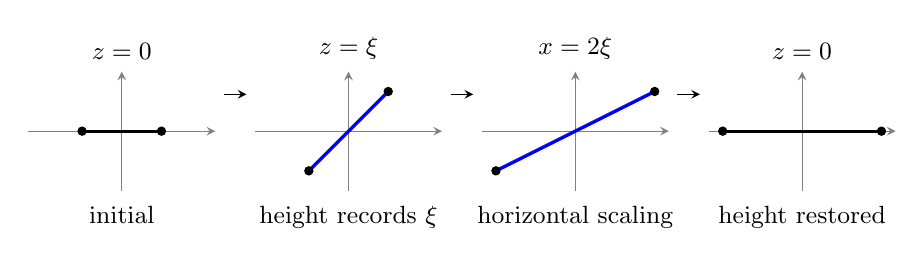
\begin{tikzpicture}[x=0.72cm,y=0.72cm,>=stealth]
\foreach \dx/\lab in {0/{initial},4/{height records $\xi$},8/{horizontal scaling},12/{height restored}}{
 \begin{scope}[shift={(\dx,0)}]
 \draw[->,gray] (-1.65,0)--(1.65,0);
 \draw[->,gray] (0,-1.05)--(0,1.05);
 \node[below,align=center,font=\small] at (0,-1.15) {\lab};
 \end{scope}}
\draw[very thick] (-0.7,0)--(0.7,0);
\draw[very thick,blue] (3.3,-0.7)--(4.7,0.7);
\draw[very thick,blue] (6.6,-0.7)--(9.4,0.7);
\draw[very thick] (10.6,0)--(13.4,0);
\foreach \x/\y in {-0.7/0,0.7/0,3.3/-0.7,4.7/0.7,6.6/-0.7,9.4/0.7,10.6/0,13.4/0}
 \fill (\x,\y) circle (1.7pt);
\draw[->] (1.8,0.65)--(2.2,0.65);
\draw[->] (5.8,0.65)--(6.2,0.65);
\draw[->] (9.8,0.65)--(10.2,0.65);
\node[above,font=\small] at (0,1.1) {$z=0$};
\node[above,font=\small] at (4,1.1) {$z=\xi$};
\node[above,font=\small] at (8,1.1) {$x=2\xi$};
\node[above,font=\small] at (12,1.1) {$z=0$};
\end{tikzpicture}
\caption{A slice of the sheet-scaling triple, in local coordinates with
vertical coefficient one and horizontal factor $\lambda=2$.  A vertical shear records the initial horizontal
offset in height; the horizontal shear doubles that offset; the last
vertical shear returns the sheet to height zero.  Nearby normal offsets
are contracted by $1/2$, as the determinant-one formula in the text shows.
Each depicted segment is the image of the entire initial segment.}
\label{sv:normal-figure}
\end{figure}


\paragraph{Evacuating before delivery.}
For $N$ rectangle maps schedule $13N$ pulses inside $[1/4,3/4]$.
First lift each source sheet to five, shift by $(4,0)$, and lower
it into storage at height two.  After all sources have been evacuated,
process them in order: lift the stored sheet, translate its center to
$v_*$, perform the six phases \eqref{sv:storage-triple}, translate
to its target center, and lower.  These passes take three and ten
phases per sheet.  The maps may send a source onto another source:
the preliminary evacuation ensures that every target footprint is free
when delivery begins.

Every resting sheet has height two and second coordinate in $[2,3]$.
During evacuation, the other resting sheets are unprocessed sources
or stored sheets; during delivery, they are stored sheets or completed
targets.  The within-family gaps and the separation between the coding
and storage squares therefore keep each vertical support off all other
resting footprints.  The correcting row has second coordinate in the
$d$-collar of $[6,7]$ and misses the resting sheets.  Horizontal transport
is supported near heights five and eight.  The $H_j$ profiles are
supported near second coordinate six and the $B$ profile near height
five.  Thus all processing pulses fix every resting sheet.  All supports
in the dependent coordinates and all moving paths are interior to the side-ten chart;
periodic copies create no further intersection.  By induction through
the slots, the full source sheets have precisely their prescribed
affine images.  The preliminary evacuation is what permits arbitrary
intersections between the source and target families.

Repeat this finite sequence from time zero and apply
Lemma~\ref{sv:force}.  Every phase is transverse and mean zero, and
the rational data and fixed smooth profiles make the construction
effective.  This proves Theorem~\ref{sv:sheet-theorem}, including
its bounded-derivative, zero-pressure, and periodicity conclusions.

\paragraph{A bound for every intermediate position.}
The same geometry gives a useful observation rule for each moving point.
Whenever the height
lies in $(3/2,5/2)$, the first coordinate belongs to
\begin{equation}\label{sv:height-guard}
 \{x^-,x^-+4,x^+\},
\end{equation}
where $x^-,x^+$ are that point's source and target first coordinates.
Horizontal transport takes place at height five and scaling in
$[9/2,11/2]$; in the indicated low band only waiting and vertical
motion occur over the source, storage point, or target.  This proves
\eqref{sv:height-guard} throughout the period.

\subsection{A separator-stack application and its observer}
\label{sv:separator}
We now supply rectangle data to the sequential construction.  The
recorder separates a finite left working word from its retained history.
A prefix rule $(s;\alpha,\beta)\to(s';\bar\alpha,\bar\beta)$
replaces the two indicated finite stack prefixes and retains both
arbitrary infinite tails.  Normalize the original machine to one halt label,
and let $A$ be its tape alphabet, with blank $b_0$. Use the stack
alphabet $A\sqcup\{\bot,\diamond\}\sqcup\{\eta_i\}$ and controls
$R_q,T_i,S_p$. At a ready control $R_q$, the left stack has the form
$L=\ell\bot H$, with $\ell\in A^*$ listing the working cells to
the left of the head, nearest first, and implicit blanks beyond them.
The separator $\bot$ keeps these cells above the retained history $H$;
the right stack begins with the scanned cell. A temporary symbol
$\diamond$ marks the beginning of the updated right working word while
$T_i$ transfers the finite left word onto that stack above the marker.
The control $S_p$ then
restores that word until $\diamond$ is exposed and removed. A new symbol
$\eta_i$ retained below $\bot$ records the instruction case.
In the transfer and restore rules, $c$ ranges over $A$.
Give each applicable case of an original instruction
$(q,a)\mapsto(p,b,d)$ its own index $i$, with $p(i)=p$, and use
\begin{equation}\label{sv:separator-primary}
\begin{array}{c|l}
d=0 &(R_q;\varnothing,a)\to(T_i;\varnothing,\diamond b),\\
d=1 &(R_q;\varnothing,a)\to(T_i;b,\diamond),\\
d=-1, c\in A &(R_q;c,a)\to(T_i;\varnothing,\diamond cb),\\
d=-1,\ \text{empty left}&(R_q;\bot,a)\to(T_i;\bot,\diamond b_0b).
\end{array}
\end{equation}
Complete the table with
\begin{equation}\label{sv:separator-transfer}
\begin{aligned}
(T_i;c,\varnothing)&\to(T_i;\varnothing,c),&
(T_i;\bot,\varnothing)&\to(S_{p(i)};\bot\eta_i,\varnothing),\\
(S_p;\varnothing,c)&\to(S_p;c,\varnothing),&
(S_p;\varnothing,\diamond)&\to(R_p;\varnothing,\varnothing).
\end{aligned}
\end{equation}
Initialize with $(R_{q_0},\bot b_0^\infty,wb_0^\infty)$.
At a ready state with $L=\ell\bot H$, the primary rule yields
$(T_i,\ell'\bot H,\diamond Y')$ with
the correct updated tape.  The transfer moves $\ell'$ right in
reverse order, inserts $\eta_i$ below $\bot$, and the restore
returns precisely those work symbols until $\diamond$ is exposed
and removed.  The new ready configuration is
$(R_{p(i)},\ell'\bot\eta_iH,Y')$, after
$2|\ell'|+3$ rules.  This is finite and positive, including an empty
left word.  Its special left-move case exposes an implicit blank correctly.
The retained instruction-case records also determine the displacement
history if absolute indexing is desired.

The source families are disjoint by tested control and top symbol.
Into $T_i$, the unique primary arrival has right top $\diamond$;
loop arrivals have distinct real symbols.  Into $S_p$, transfer
arrivals have left prefix $\bot\eta_i$, while loops have real
left top; record indices and symbols distinguish their respective cases.
There is one incoming rule into each $R_p$.  This proves disjoint
image cylinders on arbitrary tails and gives their inverses.

Use a common digit dictionary for controls and stack symbols.  If there
are $m$ entries other than the halt control, let $K=8(m+1)$,
give them distinct digits $2,4,\ldots,2m$, and give the halt control
digit $3K/4$.  Set $e(v)=\sum_jd(v_j)K^{-j}$ and
$I(v)=[e(v),e(v)+K^{-|v|}]$ for finite prefixes.  The code is
\[
 (s,L,Y)\longmapsto (2+e(sL),2+e(Y),2)\in\mathbb T_{10}^3.
\]
For a rule $(s;\alpha,\beta)\to(s';\bar\alpha,\bar\beta)$,
its rectangles are
\[
 P_i=(2+I(s\alpha))\times(2+I(\beta)),\qquad
 Q_i=(2+I(s'\bar\alpha))\times(2+I(\bar\beta)).
\]
Both families are separated in $[2,3]^2$.  Their affine factors are
$K^{|\alpha|-|\bar\alpha|}$ and
$K^{|\beta|-|\bar\beta|}$; the control digit cancels in the
first ratio.  Nonhalt first coordinates are at most
$2+(2m+1)/K<9/4$, while halt codes are between $11/4$ and $3$.
The initial code is rational by summing the blank tails.

These rectangles and maps satisfy every hypothesis of the sequential
construction in Section~\ref{sv:storage}.  Load $(2,2,2)$ horizontally
to the rational initial code during $[0,1]$, then repeat its schedule.
The fixed event is
\[
 5/2<x<7/2,\qquad 3/2<z<5/2.
\]
A halt code is in this set, including an initially halted input after
loading.  In a nonhalting run the loader has $x<9/4$.  During every
later period both endpoint coordinates lie in $[2,9/4)$;
\eqref{sv:height-guard} makes the low-height first coordinate either
less than $9/4$ or at least six.  At other heights the event is
excluded by its height condition.  Thus there is no false intermediate
hit even though an upper horizontal route may cross the observer's
projection.  Idle collars make each integer-time halt witness persist
on an interval.

Direct transverse forcing has zero pressure and is periodic after loading
at the specified side-ten viscosity.  The logarithmic choice of
Lemma~\ref{bcs:clock} instead has
$\|f(t)\|_\infty=O((1+t)^{-1})$, bounded mixed derivatives,
and $f\in L^2([0,\infty)\times\mathbb T_{10}^3)$ with the
same event.  This is a separate choice of forcing.  Under the
time-preserving scale change \eqref{sv:torus-rescale}, the label is
$(1/5,1/5,1/5)$ and the event is
$1/4<x<7/20$, $3/20<z<1/4$, with the viscosity transformation
stated there.

\subsection{Prefix rules with retained instruction tags}
\label{sv:tags}
The next recorder retains history as tags between the work symbols.
Its rectangles will be arranged in a narrow strip so that a simultaneous
construction can contract, translate, and expand all branches together.
Let $\Sigma$ be the machine alphabet, with blank $\beta$.
Replace a real tape symbol by $(a,o)\in\Sigma\times\{0,1\}$,
where $o$ marks the original cell zero and is preserved by every write.
Write the enlarged transition as $(q,a)\mapsto(q',b,d)$, with
$d\in\{+,0,-\}$.  Use controls $M(q,e)$ for
$e\in\{\star,+,0,-\}$ and $P_+(q),P_-(q)$.
For every nonhalting main control $s=M(q,e)$ and real symbol $a$
introduce a distinct tag $\gamma_{s,a}$.  The stack alphabet
$\mathcal A$ is the disjoint union of these tags and the real symbols.
At a main control $M(q,e)$, erasing all tags gives the two tape halves:
the left stack lists cells to the left of the head, nearest first,
and the right stack begins with the scanned cell. The control index $e$ records
the preceding move, with $\star$ reserved for initialization.
The transfer controls $P_+(q)$ and $P_-(q)$ finish a right or left
move by passing intervening history tags until the next real work
symbol is available. Thus history occupies space in the stacks without
being mistaken for a work cell.

A prefix rule $[s;\ell,r]\to[s';\ell',r']$ replaces the two
displayed prefixes, retaining arbitrary infinite tails.  For each main
instruction use
\begin{equation}\label{sv:tag-primary}
 [s;\varnothing,a]\longrightarrow
 \begin{cases}
 [P_+(q');b\gamma_{s,a},\varnothing],&d=+,\\
 [P_-(q');\varnothing,b\gamma_{s,a}],&d=-,\\
 [M(q',0);\varnothing,b\gamma_{s,a}],&d=0.
 \end{cases}
\end{equation}
For every tag $g$ and real symbol $c$ include
\begin{equation}\label{sv:tag-transfer}
\begin{aligned}
{}[P_+(q);\varnothing,g]&\to[P_+(q);g,\varnothing],&
[P_+(q);\varnothing,c]&\to[M(q,+);\varnothing,c],\\
[P_-(q);g,\varnothing]&\to[P_-(q);\varnothing,g],&
[P_-(q);c,\varnothing]&\to[M(q,-);\varnothing,c].
\end{aligned}
\end{equation}
Initialize in $M(q_0,\star)$ with an unmarked blank left stack and
the input followed by blanks on the right, marking the right top as
the origin (a marked blank for empty input).

For a right move, the primary rule pushes the written symbol left and
the transfer removes any tags above the next real right symbol.
For a left move, it writes the new right top, removes tags from the
left, and moves its next real symbol onto the right.  A stay just writes
and inserts its tag.  Each original instruction adds exactly one tag;
at every finite stage there are only finitely many tags to transfer.
After $j$ prior machine steps, the next step takes one rule for a stay
or two plus the number of transferred tags for a nonzero move, hence
at most $j+3$ rules.  If $n_k$ is the rule count after $k$ machine
steps, then
\[
 k\le n_k\le k(k-1)/2+3k.
\]
No intermediate control is terminal.  The origin flag recovers the
absolute head position: it is $k$ when the mark is the $k$th real
symbol of the left stack and $1-k$ when it is the $k$th of the right.

Both rule-cylinder families are disjoint on arbitrary tails.  Source
controls and tested top symbols distinguish rules.  Into $P_+(q)$,
primary arrivals have left prefix $b\gamma_{s,a}$ beginning with a
real symbol, while loops have a tag there.  Distinct tags distinguish
the primary arrivals.  The analogous argument on the right applies
to $P_-(q)$.  Exits into $M(q,+)$ or $M(q,-)$ have distinct
real right top symbols, while arrivals into $M(q,0)$ have distinct
two-symbol prefixes $b\gamma_{s,a}$.  No rule enters a star-tagged
main control.  These tests also invert each rule; they do not assume
that the tails encode an initialized computation.

Let $K$ be the number of controls, set $\lambda=1/(16(K+1))$,
and enumerate nonhalting and halting controls separately from zero.
Place their origins at
\[
 (A_s,1/4),\qquad A_s=\xi_s+(2j_s+1)\lambda,
 \qquad \xi_s=\begin{cases}1/8,&s\text{ nonterminal},\\
 11/16,&s\text{ terminal}.\end{cases}
\]
Use odd digits in base $B=2|\mathcal A|+1$ for the stack alphabet.
A prefix $w$ acts on its free tail parameter by
$F_w(t)=\sum_jd(w_j)B^{-j}+B^{-|w|}t$, with interval
$I(w)=F_w([0,1])$.  Hence each prefix rule gives a positive diagonal
map from
\[
 (A_s+\lambda I(\ell))\times(1/4+\lambda I(r))
 \quad\hbox{to}\quad
 (A_{s'}+\lambda I(\ell'))\times(1/4+\lambda I(r')).
\]
The factors are $B^{|\ell|-|\ell'|}$ and
$B^{|r|-|r'|}$.  At the first conflicting digit the closed intervals
have a positive gap; the full-cylinder argument therefore gives
separately disjoint closed rectangle families.  It imposes no condition
on a source intersecting a target.  Constant-tail sums give the rational
initial code.

\subsection{Fifteen simultaneous phases}
\label{sv:fifteen}
We use the rectangles just constructed in Section~\ref{sv:tags},
on the unit torus.  Both families are separately separated, every
half-width is at most $\lambda/2<1/2$, and all second coordinates lie
in $[1/4,1/4+\lambda]$.  These are the geometric properties needed
for the simultaneous construction; source--target intersections remain
allowed.  Write the source and target rectangles as
$D_i=p_i+[-s_{i1},s_{i1}]\times[-s_{i2},s_{i2}]$ and
$T_i=q_i+[-t_{i1},t_{i1}]\times[-t_{i2},t_{i2}]$.
Choose symmetric product cutoffs $\chi_i^D,\chi_i^T$ on
neighborhoods, separately disjoint, with collars smaller than $1/32$.
The original supports lie in the common strip
$1/4-1/32<y<1/4+\lambda+1/32$; their translates by
$\omega=(0,1/2)$ therefore miss all tracked rectangles and all
untranslated supports.  For $N>0$ branches
put
\[
 z_\circ=1/2,\quad z_i=1/4+\frac{i}{2(N+1)},\quad
 d=\kappa=\frac1{16(N+1)},\quad
 \epsilon=\frac12\min_{i,j}\{s_{ij},t_{ij}\}.
\]
Let $\zeta_i$ be symmetric about $z_i$, one near
$[z_i-d,z_i+d]$, with support in $(z_i-2d,z_i+2d)$.
The closures of these supports are disjoint.  Define
$G_i(z)=(z-z_i)\zeta_i(z)$.  Both $G_i$ and $G_i'$ have
zero mean, by oddness and differentiation, and are respectively
$z-z_i$ and one near the required height interval.

The essential operation changes one coordinate of one sheet.  For
centers $o_i$, symmetric rectangle cutoffs $\chi_i$, and factors
$\mu_i>0$, use three successive profiles
\begin{equation}\label{sv:sheet-triple}
 e_z\sum_i\kappa(y_j-o_{ij})\chi_i(y),\qquad
 e_j\sum_i\frac{\mu_i-1}{\kappa}G_i(z),\qquad
 -e_z\sum_i\frac{\kappa}{\mu_i}(y_j-o_{ij})\chi_i(y).
\end{equation}
Starting at height $z_i$ with offset $\xi$ in coordinate $j$,
these stages give height $z_i+\kappa\xi$, horizontal offset
$\mu_i\xi$, and height $z_i$.  If $|\xi|\le1/2$ and the
horizontal segment remains in the cutoff rectangle, the height lies
in the linear plateau and no other height profile acts.  Every vertical
profile has zero mean because its linear factor is odd under reflection
about the rectangle center.  Every profile is a transverse shear.

Now lift $D_i$ from $z_\circ$ to $z_i$ using the mean-zero selector
$\chi_i^D(y)-\chi_i^D(y-\omega)$.  Use
\eqref{sv:sheet-triple} first in coordinate one and then coordinate
two, with $o_i=p_i$ and $\mu_i=\epsilon/s_{ij}$.
This takes six stages and contracts every source to
$p_i+[-\epsilon,\epsilon]^2$.  Translate by
$(q_i-p_i)G_i'(z)$.  Next apply the same two triples with
$o_i=q_i$, $\chi_i=\chi_i^T$, and
$\mu_i=t_{ij}/\epsilon$.  Finally lower using the target
selector difference.  There are $1+6+1+6+1=15$ stages.
Assign them disjoint pulse supports inside $[1/4,3/4]$.

During contraction the entire projection stays in its source rectangle;
during expansion it stays in its target rectangle.  Thus all rectangle
plateaus used in \eqref{sv:sheet-triple} remain valid, including when
the other coordinate has already changed.  The translation at height
$z_i$ is exactly by $q_i-p_i$.  Consequently the period map is
\begin{equation}\label{sv:fifteen-map}
 (y,z_\circ)\longmapsto
 \left(q_i+\operatorname{diag}(t_{i1}/s_{i1},t_{i2}/s_{i2})
                 (y-p_i),z_\circ\right),\qquad y\in D_i.
\end{equation}
For an empty rule list use zero.  As in the sequential construction,
the normal compensation follows directly from the three shears: in
the linear core a triple
acts on a small initial height deviation $\zeta$ by
\[
 (\xi,\zeta)\longmapsto
 \left(\mu_i\xi+\frac{\mu_i-1}{\kappa}\zeta,
                      \frac{\zeta}{\mu_i}\right).
\]
Its determinant is one, while its restriction to $\zeta=0$ multiplies
the horizontal coordinate by $\mu_i$.  Figure~\ref{sv:normal-figure}
shows this three-shear mechanism on a one-dimensional slice.
The sheet statement
\eqref{sv:fifteen-map} therefore permits planar area change without
claiming that a thick box has that same diagonal action.

Load the fixed label $(1/2,1/2,1/2)$ to the rational initial code
at height $z_\circ$.  A profile $G_\circ'(z)$ supplies a
mean-zero horizontal loader if $G_\circ$ equals $z-1/2$ near
$1/2$ and vanishes near the coordinate endpoints.  Run it once during
$[0,1]$, then repeat the fifteen-stage processor.  At $1+n$ the
particle represents rule $n$ by \eqref{sv:fifteen-map}.  Nonhalt
source and target rectangles have first coordinates in $(1/8,1/4)$;
contractions, expansions and the middle translation preserve that band.
Loading follows a segment from $1/2$ into that band.  Thus a
nonhalting run never enters $5/8<x<7/8$.  Terminal codes are in
$(11/16,13/16)$ and do enter it, including after loading for an
initial halt.  The finite positive rule counts proved above show that
no machine step is left indefinitely unfinished.  Direct transverse
forcing gives the smooth mean-zero solenoidal force, pressure zero,
and periodicity after loading.  The repeated processor depends only on
the transition table; the input affects only the rational loading code.

\section{The equation in material labels}
\label{sv:material}
Let $u,p$ be any smooth torus solution constructed above, and let
$X(t,a)$ be its material flow.  Put
$M(t,a)=D_aX(t,a)$ and $P(t,a)=p(t,X(t,a))$.
The smooth flow is a diffeomorphism on each finite time interval.
Differentiating its equation gives
\[
 \partial_tM=(D_xu)(t,X)M,\qquad
 \partial_t\det M=(\operatorname{div}u)(t,X)\det M=0,
 \qquad M(0,a)=I.
\]
Thus $\det M=1$.  In particular the observed particle belongs to
this volume-preserving flow of the unique solution.

For each component the equation in material labels is
\begin{equation}\label{sv:material-equation}
 \partial_{tt}X_i=-(M^{-T}\nabla_aP)_i
 +\nu\operatorname{div}_a
       (M^{-1}M^{-T}\nabla_a\partial_tX_i)
 +f_i(t,X(t,a)),\qquad \det M=1.
\end{equation}
Indeed, differentiating $X_t=u(t,X)$ yields the Eulerian material
derivative $u_t+(u\cdot\nabla)u$.  The chain rule gives
$(\nabla_xp)\circ X=M^{-T}\nabla_aP$ and
$(\nabla_xu_i)\circ X=M^{-T}\nabla_aX_{i,t}$.
To verify the order of the factors in the diffusion term, use a smooth
periodic test function $\varphi$ and volume preservation:
\begin{align*}
 \int(\Delta_xu_i)\circ X\,\varphi\,da
 &=-\int (\nabla_xu_i)\circ X\cdot M^{-T}\nabla_a\varphi\,da\\
 &=-\int M^{-1}M^{-T}\nabla_aX_{i,t}\cdot\nabla_a\varphi\,da.
\end{align*}
Periodic integration by parts proves the asserted diffusion operator;
smoothness upgrades this test-function identity to a pointwise one.
The shear constructions have $p=0$ and therefore $P=0$.
Their prescribed open-set events consequently observe the material
evolution governed by \eqref{sv:material-equation} itself.
